\chapter{Opis projektnog zadatka}
				
		\section{Uvod}
		
		Cilj ovog projektnog zadatka je razviti programsku potporu za web aplikaciju $\textit{Connectima}$ koja predstavlja inovativnu platformu za promociju raznih vrsta događanja. Aplikacija je namijenjena široj populaciji koja je zainteresirana za najavljena događanja u svojoj okolini ili želi popularizirati svoje događanje. \\ Korisnici mogu pregledavati događanja i njihove organizatore te po završetku događanja iste recenzirati. Također, organizatori događanja mogu ih objavljivati uz mogućnost dodavanja širokog spektra informacija i medijskih sadržaja.\\
		U nastavku su opisani korisnički zahtjevi i glavne funkcionalnosti ove web-aplikacije.
		
		\section{Opis funkcionalnosti}
		
			\subsection{Stranice}
			
				\subsubsection{Početna stranica}
				Pri pokretanju web aplikacije prikazuje se početna stranica. S lijeve strane stranice nalazi se navigacijska traka s različitim stranicama koje sadrže događanja, podatke o korisniku i drugo. Pošto korisnik u tom trenutku još nije autoriziran, ne može pristupiti nijednoj od dolje navedenih stranica, osim 'Prijava' i 'O nama'.
				
				\subsubsection{O nama}
				Stranica 'O nama' javno je dostupna svima, a ukratko predstavlja cilj web aplikacije i osnovne informacije.
				
				\subsubsection{Prijava}
				 Na stranici prijava korisniku se omogućuje prijava u sustav pomoću adrese elektroničke pošte i lozinke. Ako korisnik još nije registriran u sustav, na istoj se stranici može registrirati i odabrati želi li biti organizator ili posjetitelj.
				 
				\subsubsection{Događanja}
				Nakon uspješne prijave ili registracije, korisnika se preusmjeruje na stranicu s događanjima. Može ih filtrirati po vremenu održavanja te otvarati pojedina događanja kako bi dobio više informacija.\\
				Pri pregledu svih događanja prikazuju se naziv događanja, jedna slika, lokacija, vrijeme i organizator, a pri pregledu pojedinačnih događanja prikazuju se svi podaci.
				
				\subsubsection{Moj račun}
				Na stranici 'Moj račun' korisnik može pregledati i uređivati osobne podatke te odjaviti se iz sustava. Osim navedenog, korisnici koji imaju ovlasti organizatora mogu dodavati i brisati vlastita događanja te platiti članarinu. Administrator preko ove stranice može pristupiti popisu svih korisnika te upravljati njima i njihovim događanjima.
			
				\subsubsection{Moj kalendar}
				'Moj kalendar' predstavlja stranicu na kojoj korisnici mogu kronološki pregledati događaje za koje su izrazili interes i najavili dolazak.
				
			
			\subsection{Vrste korisnika}
			U sustavu postoje četiri vrste korisnika:
			\begin{packed_enum}
				\item anonimni (neregistrirani) korisnik,
				\item posjetitelj,
				\item organizator i 
				\item administrator.
			\end{packed_enum}
			
			\underline{Anonimni korisnik} ne može koristiti aplikaciju niti pregledavati njen sadržaj dok god se ne prijavi ili registrira. Može se samo upoznati sa izgledom početne stranice i pročitati osnovne informacije o aplikaciji. \\
			
			\underline{Posjetitelj} može pregledati događanja objavljena na stranici, detalje o njima i njihovim organizatorima. Može ih filtrirati po odabranom vremenskom razdoblju (24h, 7 dana, 30 dana, prošla događanja). Također, može pregledati i mijenjati osobne podatke, odjaviti se i obrisati svoj korisnički račun. Na zasebnoj stranici može pregledati događanja za koja je izrazio interes (najavio dolazak). Najaviti dolazak može za bilo koje događanje koje još nije počelo. Po završetku događanja, u roku 48 sati može ostaviti recenziju događanja. Posjetitelj također može uključiti primanje obavijesti o događanjima na nekom području ili neke određene vrste. \\
			
			\underline{Organizator} ima sve ovlasti posjetitelja. Uz to, može dodavati događanja i uređivati ih. Ne može recenzirati vlastita događanja ili najaviti dolazak na njih, ali oni mu se automatski prikazuju u kalendaru.\\
			Postoje dvije skupine organizatora: oni koji aplikaciju koriste besplatno te oni koji plaćaju članarinu. Prema osnovnim postavkama, svaki organizator na početku aplikaciju koristi besplatno. Članarinu mora platiti ako želi dodavati događanja koja nisu besplatna, već se za njih mora platiti ulaznica. \\
			
			\underline{Administrator} ima najveće ovlasti. Njegov je zadatak nadziranje podataka koji se dijele u aplikaciji, dakle događanja i korisnike. Administrator može pregledavati sve korisnike te ih filtrirati na posjetitelje i organizatore. Može obrisati korisničke račune drugih korisnika, pojedina događanja i recenzije. Postavlja i mijenja cijenu članarine. Administrator ne može obrisati svoj račun, dodavati i recenzirati događanja. 
		
		\section{Slična rješenja}
		
		Već postoje mnoge aplikacije koje imaju isti ili sličan cilj kao i naša aplikacija. \\
		Društvene mreže poput Facebooka omogućavaju dodavanje događanja koja se mogu dijeliti na profilu korisnika. S događanjem mogu se povezati naknadne objave korisnika, lokaciju događaja moguće je vidjeti na karti te se, kao i na našoj stranici, može pronaći sve potrebne informacije o samom događanju, ali i njegovom organizatoru. 
		
		\begin{figure}[H]
			
\includegraphics[scale=0.7]{slike/Facebook_dogadanja.png}
			\centering
			\caption{Primjer događanja oglašenog na Facebooku}
		\end{figure}
		
		Iako naša aplikacija u ovoj fazi još ne posjeduje sve te funkcionalnosti, svakako ima prednosti pred navedenom opcijom na Facebooku. Facebook je društvena mreža kojoj oglašavanje događanja nije primarni cilj. Mnogi korisnici žele pratiti događanja u blizini te ista dodavati bez da pritom kreiraju profil na nekoj društvenoj mreži. Upravo je to prednost naše aplikacije koja služi isključivo za promociju događanja.\\
		
		Drugi je primjer aplikacija \textit{Meetup}. Meetup je po većini funkcionalnosti vrlo sličan našoj aplikaciji. Događanja se mogu filtrirati po lokaciji i vremenu. Dodatna funkcionalnost s obzirom na \textit{Cennectimu} je mogućnost prijave na događanje. Upravo je u tome ključna razlika između ove dvije aplikacije. \textit{Connectima} je zamišljena kao aplikacija za sve vrste događanja, od malih lokalnih okupljanja do velikih koncerata i konferencija. \textit{Meetup} je, s druge strane, aplikacija specijalizirana za konferencije i radionice koje zahtijevaju raniju najavu.
		 
		\begin{figure}[H]
			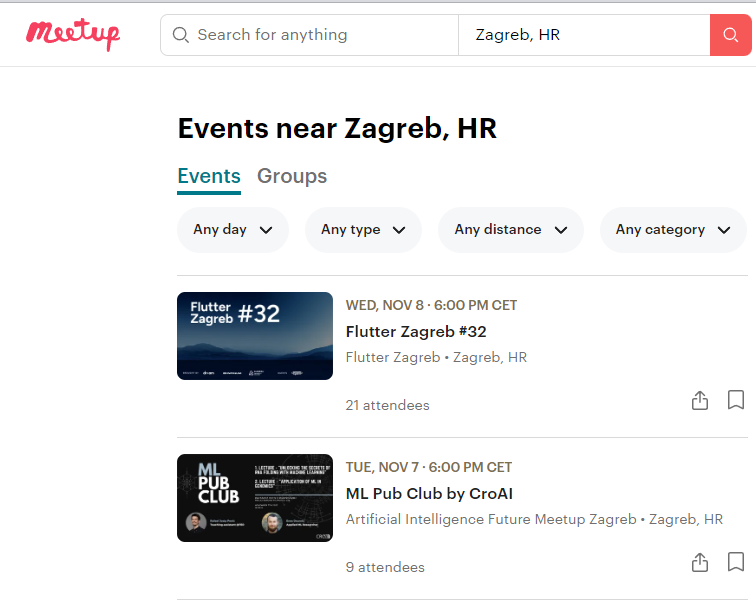
\includegraphics[scale=0.7]{slike/Meetup.png}
			\centering
			\caption{Početna stranica aplikacije Meetup}
		\end{figure}
		
		\section{Moguće nadogradnje}
		
		Ova aplikacija ima još puno prostora za nadogradnju pa bi iduće verzije mogle uključivati:
			
			\begin{packed_enum}
				\item uvođenje dodatnih jezika aplikacije (engleski, njemački...),
				\item integraciju s popularnim društvenim mrežama i aplikacijama za razmjenu poruka (Facebook, Instagram, Whatsapp, Viber) za jednostavno dijeljenje događanja
				\item dodatne načine plaćanja
				\item umetanje medijskih sadržaja uz recenziju
				\item preuzimanje događanja u vlastiti kalendar u iCal formatu
				\item pretragu događanja na interaktivnoj karti
				\item mogućnost razmjena poruka među korisnicima
			\end{packed_enum}
			
		Uz sve navedeno, dodatne bi se funkcionalnosti mogle dodavati na temelju povratnih informacija svih korisnika (posjetitelja, organizatora i administratora).
		
		\eject
		
	